\documentclass[11pt]{article}
% packages
% Fran Burstall's Bath thesis package
\usepackage{baththesis}
\usepackage{amssymb} %for Blackboard bold etc \usepackage{graphicx} %for including eps graphics % front matter
\usepackage[pdftex]{graphicx} % To include pictures
\usepackage{caption}
\usepackage{subcaption} % To use subfigures with subcaptions
\usepackage{url}
\usepackage{amsmath} % Equations
\usepackage{txfonts}
\setlength{\parskip}{0.9em} %Paragraph spacing
\usepackage{pgfgantt}
\usepackage{cite}
\usepackage{csquotes}
\usepackage[ruled]{algorithm2e} % Algorithms 
\renewcommand*{\mkcitation}[1]{ #1}

\newcommand{\phim}{\mathbf{\phi}}
\newcommand{\X}{\mathbf{X}}
\newcommand{\x}{\mathbf{x}}
\newcommand{\Y}{\mathbf{Y}}
\newcommand{\y}{\mathbf{y}}
\newcommand{\w}{\mathbf{w}}
\newcommand{\Z}{\mathbf{Z}}
\newcommand{\z}{\mathbf{z}}
\newcommand{\h}{\mathbf{h}}
\newcommand{\dd}{\: \mathrm{d}}

%\usepackage[hidelinks]{hyperref} % Adds references links without color
\usepackage{hyperref} % Adds references links with color
\usepackage{xcolor}
\hypersetup{
    colorlinks,
    linkcolor={red!50!black},
    citecolor={blue!50!black},
    urlcolor={blue!80!black}
}

\title{Visual Effects} \author{Ieva Kazlauskaite, Garoe Dorta-Perez, Richard Shaw}
%\degree{Doctor of Philosophy}
\unit{ unit }
\department{Department of Computer Sciences} \degreemonthyear{May 2015}
\norestrictions

\begin{document}
\maketitle

\section{Introduction}
\label{ch:intro}
\begin{center}
\textquote[~\cite{Attenborough:1998}]{\textit{Birds are the most accomplished aeronauts the world has ever seen. They fly high and low, at great speed, and very slowly. And always with extraordinary precision and control}.}
\end{center}

A talented painter or sculptor is able to imagine and reproduce the subtle details of a human face. Hours of training and endless manual adjustments are required before an arbitrary shape resembles a facial expression. Furthermore, a human eye is trained to notice subtle changes in the expression of another human being, which also applies to animated humans, thus even the smallest discrepancies in an animated model are easily detected. Though artists are able to produce good quality and appealing results, the limitations in budget and time so prominent in the entertainment industry motivate the development of more automated, faster and cheaper models.

The naive approach that allows for faster performance is the keyframe animation; though it is still based on manual input, keyframe animation requires fewer frames as the intermediate expressions are interpolated over. However, this approach is still very laborious and time consuming. With the emergence of software and systems for motion capture, development of mathods for performance-driven animation has received significant attention from both the industry as well as the academia.



%-----------------------------------------------------------------------
\section{Previous Work}
\label{sec:previous}

\subsection{Data Capture}

%-----------------------------------------------------------------------
\subsection{Sparse Reconstruction}


%-----------------------------------------------------------------------
\subsection{Facial Animation}
The first attempts at using performance-driven facial animation in academia date back to late $20^{th}$ century while in industry was first used for guidance rather than production, i.e. the facial motion of Gollum in the \textit{Lord of the Rings} was based on the motion capture data of the performance of the role actor Andy Serkis~\cite{Pighin:2002}. Another notable example is the pipeline used in the making of \textit{the Polar Express}; the motion capture data was used to construct a multilayer facial rig that was used by an artist to create the final animation~\cite{Bennett:2005}. Though many other examples exist, often the exact technology and methods used in production are not disclosed.

In the last two decades, nearly two hundred academic papers that include words \textit{face}, \textit{animation} and \textit{motion capture} were published in computer graphics and vision journals ~\cite{Scopus}. The increase in the quality of the results is explained by the advancements in both the capturing technology and the computational methods. We shall concentrate on the latter; for a brief discussion of the capturing methods see Sec.~\ref{sec:datacapture}. 

The work of Guenter et al. provides the first detailed and unified system for capturing and reconstructing facial performance~\cite{Guenter:1998}. Their work is mostly focused on motion tracking and production of labelled three-dimensional motion of the dots on the actors face. Once a sequence of  moving dots is acquired, the authors scan the actors face to get a polygonal mesh that corresponds to the geometry of the face. The motion of the sparse dots is described in terms of offsets from the neutral position. Then the vertices in the mesh are moved by calculating a linear combination of the offsets of the nearest dots, i.e. in each frame a weighted sum of the change in the dot position is calculated and added to the neutral position of the given vertex. The weights are chosen to be zero everywhere except in the one-ring neighbourhood where the weights depend on the distance of the vertex to the dots; the weights must sum to one. An additional stationary ring of dots is added on the edge of the face to ensure there is no motion outside the face. The algorithm suffers from noise introduced during in the tracking, the reconstruction and the three-dimensional scanning. Moreover, the choice of the nearest dots for each vertex in the mesh is not trivial due to the irregular distribution of the tracked dots. The method that assigns the blends has a number of manually adjusted parameters and does not guarantee to find the best set of reference dots. Additionally, the areas around the eyes and lips require a special treatment; the dots above and below the problematic areas are marked and are not allowed to be blended. The authors point out that a number of artefacts are visible in the resulting animation; some of these flaws attributed to the poor quality of the facial scan, and the fact that the reconstruction method is not robust to jitter and  incorrect placement of the tracked data.


%-----------------------------------------------------------------------
\subsection{Skin Rendering}

Rendering realistic skin is a challenging task.
As social beings we interact with interact with other individuals on a daily basis, which has made human perception quite sensitive to skin appearance, even more so with human faces.
Skin is composed of several layers with different properties, to accurately simulate skin the light transport between this layers has to be simulated.
The full effect of light scattering between two points on the surface can be modelled using a Bidirectional Surface-Scattering Distribution Function (BSSRDF).

Weyrich et al~\cite{Weyrich2006} proposed a two-layer model for skin rendering, the outer layer simulates the air-oil interface and the inner layer models the subsurface scattering in the skin.
The authors considered the scattering to be homogeneous, with this assumption they measured the skin BRDF of several subjects in a light dome, while the scattering was sampled at three points in the face with a custom made sensor.
The BRDF data was fitted to a Blinn-Phong and a Torrance-Sparrow isotropic models, and the scattering was fitted with a single transport coefficient.
Donner et al~\cite{Donner2008} also proposed a two-layer model, however the authors allow for the layers to be heterogeneous.
With this addition they are able to introduce the effects of haemoglobin, veins and tattoos.
Emotional induced haemoglobin variations have also been explored ~\cite{Jimenez2010}.
The authors measured the haemoglobin distributions of several subjects in different poses, then a linear combination of the captured data would determine the final haemoglobin distribution for a new sequence.
Recently, Iglesias et al~\cite{Iglesias2015} introduced a five-layer model to handle skin ageing.
Haemoglobin, collagen and fat changes with age are modelled using the different layers.

Normal maps are use to alter the normals of the scene objects during rendering.
This technique is used to add geometric detail to an object at rendering time without actually changing the geometry.
%The error introduced with this approach is shown in Figure \ref{fig:normal_map}, a ray $r_1$ hist the geometry at point $p$ and the normal $n_p$ is used for shading, while if we had the based geometry the hitting point would be $p'$ and the normal $n'$.
Normal maps for skin rendering are usually captured using expensive light domes with a number of synchronized cameras ~\cite{Graham2013, Weyrich2006}. 

Another technique to increase the quality of a face render is to scale the resolution of the textures being used.
Ashikhmin et al~\cite{Ashikhmin2001} presented a method to generate new textures using a goal image by greedily extending existing patches whenever possible.
Hertzmann et al~\cite{Hertzmann2001} extended Ashikhmin et al~\cite{Ashikhmin2001} method by adding a second example image and using more complex distance metric to choose the next synthesized pixel.
Graham et al~\cite{Graham2013} applied Hertzmann et al~\cite{Hertzmann2001} example-based filter to generate bump maps with increased quality for skin rendering.
An alternative approach using a dictionary of samples was presented by Jianchao et al~\cite{Jianchao2010}.
This method is restricted to generating super-resolution images, however, the previous methods support a wide variety of filter effects.
For an in depth analysis of super-resolution techniques, we refer the readers to Tian et al~\cite{Tian2011} survey.

%\begin{figure}[htbp!]
%\centering
%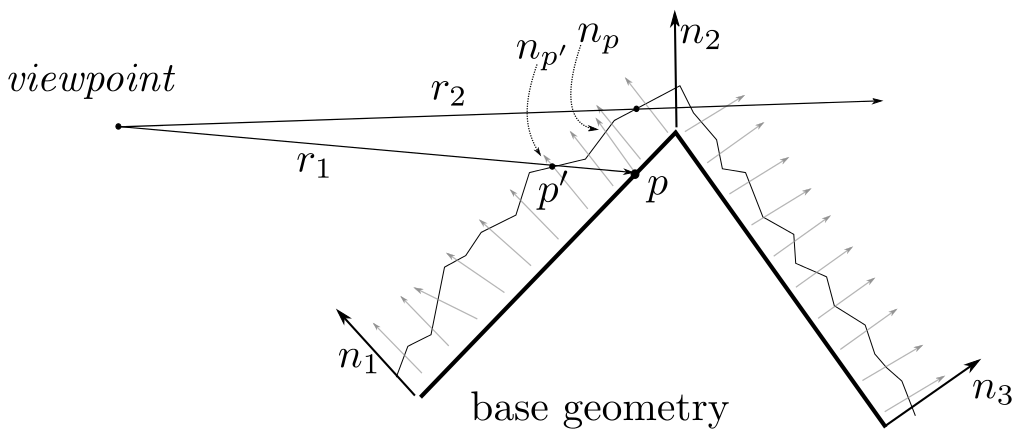
\includegraphics[width=0.7\textwidth]{img/normal_map}
%	\caption{ Using normal maps to simplify a given geometry, image taken from \cite{ganovelli2014}.}
%	\label{fig:normal_map}
%\end{figure}



%-----------------------------------------------------------------------
\section{Methodology}
\label{sec:methods}


\subsection{Data Capture} \label{sec:datacapture}


\subsection{Sparse Reconstruction}


\subsection{Blendshape Optimisation}
In this section we introduce the techniques used to warp the meshes, and the optimisation methods.

\subsubsection{Thin Plate Splines}
Thin plate theory deals with problems that commonly arise in areas of natural sciences and engineering when trying to model the behaviour of a thin sheet of some material. The possible processes include but are not limited to stretching, bending, crumpling, buckling, shrinking, straining and tearing. The corresponding mathematical model is based on ideas from differential geometry, and the set of equations describing the aforementioned phenomena are often notoriously difficult to solve. Therefore, in Computer Graphics, as well as other fields, a number of simplifying assumptions are made when constructing a thin plate model. 

A thin plate is considered to be a two dimensional object, i.e. it is assumed that the thickness is infinitesimal. The geometry of the object is often simplified to reduce the computational cost. Thin plate splines (TPS) are a two-dimensional counterpart of the cubic spline~\cite{Sibson:1991}. TPS are a deformation method based on the assumption that a thin surface deforms in a way that minimises the surface bending energy. The bending energy is proportional to the change in the second fundamental form. Specifically, given two corresponding sets of point $\{(x_i, y_i\}_i^N$ and $\{v_i\}_i^N$ there exists a height field mapping between the two, $f: \mathbb{R}^2 \to \mathbb{R}$. The bending energy corresponding to this mapping is proportional to the second order derivatives of the mapping:
\begin{equation}
\begin{aligned}
	E_{bend}(f) = \lambda \iint \left( \left( \dfrac{\delta^2f}{\delta x^2} \right)^2 +  2 \left( \dfrac{\delta^2f}{\delta x y} \right)^2 +  \left( \dfrac{\delta^2f}{\delta y^2} \right)^2 \right) \dd x \dd y,
\end{aligned}
\end{equation} where $\lambda$ is smoothing parameter, which balances the quality of fit and the amount of bending, i.e. the wiggliness of the function. TPS finds the transformation that fits the data while minimising the bending energy. Note that TPS may also be defined in terms of the radial basis functions that are used for smooth scattered data fitting. The RBF solution for thin plate splines is:
\begin{equation}
\begin{aligned}
	f(x,y) = \sum_{i=1}^N \omega_i \: \phi(\|(x,y) - (x_i,y_i)\|), \: \text{ where} \: \phi(r) = r^2 \log(r).
\end{aligned}
\end{equation} To ensure that the function $f$ has square-integrable second derivatives, the following conditions are imposed:
\begin{equation}
	\sum_{i=1}^N \omega_i = \sum_{i=1}^N \omega_i x_i = \sum_{i=1}^N \omega_i y_i = 0.\label{eq:TPSrestrictions}
\end{equation} These conditions and the data fitting requirement may be combined into a linear system of equations:
\begin{equation}
\begin{bmatrix}
	K & P \\
	P^T & 0 
\end{bmatrix} 
\begin{bmatrix}
	\omega \\
	o
\end{bmatrix} = 
\begin{bmatrix}
	v \\
	o
\end{bmatrix}, 
\end{equation} where $K$ encodes the relation between the data points, i.e. $K_{ij} = \phi(\|(x_i,y_i) - (x_j,y_j)\|)$, $P_{i\cdot} = (1, x_i, y_i)$ contains the variables from Eq.~\ref{eq:TPSrestrictions}, $\omega$ contains the values of $\omega_i$, and $v$ contains the target function values $v_i$. The variables $0$ and $o$ denote the zero matrix and the zero column vector respectively. Solving this linear system of equations gives the desired transformation in two dimensions. The method extends naturally to three-dimensional problems by including a dependence on an additional variable in the calculations described above.

\subsubsection{Non-Rigid ICP}
Iterative Closest Point (ICP) is an algorithm used to align two partially overlapping point clouds by minimising the square error between corresponding points. The quality of the results produced by this algorithm is sensitive to the initial guess at a solution, i.e. ICP only refines the initial estimation. See Alg.~\ref{alg:icp} for the outline of the algorithm. Mean square error algorithm is used to calculate the average of the squared errors between the target and the transformed source points. Thus the objective function is a function of rotations and translations. The output of the algorithm is a transformation matrix that provides the optimal mapping between the two point clouds within a given threshold. The transformation matrix may be split into rotation and translation. The algorithm solves a linear system of equations where the unknowns are the coefficients in the rotation matrix and the translation vector and the known point cloud values are used as coefficients. The method is often used to find a transformation between a point cloud and a surface; in that case the surface normals are used as additional input.

\begin{algorithm}[H]   \caption{Iterative Closest Point.}
\KwData{source point cloud \\
\hspace{0.9cm} target point cloud\;
\hspace{0.9cm} initial guess\;
\hspace{0.9cm} error threshold\;
 }
\BlankLine
\While{error $>$ threshold}{
\For{point in source}{
  find closest point in target\;
  }
use mean squared error to find best transformation that aligns source to target \;
apply transformations\;
}
 \label{alg:icp}
\end{algorithm} 
The original ICP algorithm is limited to rigid transformations, i.e. rotation and translation, which have only $6$ degrees of freedom. However, in order to capture scaling, shearing and other more complicated transformation, an affine mapping should be used. Thus an extension of the ICP algorithm, called non-rigid ICP is used when additional degrees of freedom are present. Allen et al. proposed a non-rigid registration method that uses a numerically non-linear solver to find a smooth affine mapping~\cite{Allen:2003}. Additional constrained are imposed by manually matching some known marker locations in the two datasets. The method exhibits slow convergence and often leads to local minima; consequently, the authors use a multi-resolution approach where the optimisation is first performed on a low resolution mesh, and then optimised on the high resolution mesh. Amberg et al. combined the ICP algorithm with the method of Allen et al. to overcome the issues with convergence~\cite{Amberg:2007}.

\subsubsection{Blendshape model}
The aim of this project is to used captured data of a face to animate a given model. We use the digital Emily model that comes with $68$ controllable blendshapes ranging from simple eyebrow movements to complicated lip corner pulls. Each blendshape has a weight $w_i$ associated with it, and $w_i \in [0,1]$. The model includes eyes and teeth. The aim is to find a combination of these blendshapes that produce a specified facial expression. In particular, we are interested in reproducing the captured sequence of expressions. 

\textbf{First attempt}. We manually construct a sparse set of points that corresponds to the sparse source mesh. Then the neutral expression of the subject is matched with the neutral expression of Emily by transforming the sparse source mesh to the sparse target mesh. The transformation is then stored, and it is used to map all the expressions in the captured sequence. This produces a sparse Emily sequence; using TPS again we warp the dense Emily mesh according to the positions of the sparse points. The quality of the resulting animation is poor for a number of reasons, see Fig.\ref{}. Firstly, the sparse points are not able to constrain the dense mesh, especially since parts of the face, for example the eyelids and the lips are not tracked in the sparse mesh. Consequently, numerous artefacts appear on the dense mesh, and they are particularly noticeable around the lips as no boundary conditions are imposed. Secondly, though there is a clear correspondence between the generated Emily sequence and the source sequence, the generated expressions look unnatural. This may be explained by the differences in the geometry and anatomy of the two faces; for instance, the source may be able to pull expressions that may not be mimicked by the model. In addition, the errors in tracking, reconstruction, and manual selection of sparse points on Emily further reduce the quality of the animation.

\textbf{Simplified mesh}. Our initial attempt to improve the method involved simplifying the dense Emily model by removing the part of the mesh that corresponds to the lips. Though the simpler mesh exhibited slightly better behaviour, i.e. there were fewer visible artefacts, the sparse point cloud was still unable to constrain the dense mesh well enough to produce realistic results, see Fig.~\ref{}. 

\textbf{Introduction of blenshapes}. In an attempt to improve the visual appeal of the generated animation, we decided to use a set of Emily key-shapes, that were readily available to us. The main argument for using these 

A number of different numerical optimisation methods where tested when solving for the blendshape  weights.

\subsection{Skin Rendering}

Our objective in skin rendering is to generate a face that would be indistinguishable from a real one.
In our case, we have have taken a 3D scan of a subject and our aim is to improve the realism when rendering it.
For this task we will mainly look at the techniques presented by Hertzmann et al~\cite{Hertzmann2001} and Graham et al~\cite{Graham2013}.

Before we begin, lets explain the Image Analogies framework~\cite{Hertzmann2001} in more detail.
Given three images $A$, $A'$ and $B$, where $A$ is an unfiltered example, $A'$ is a filtered example, and $B$ is an input image, the algorithm will generate an output image $B'$ such that $B'$ relates in the same way to $B$, as $A'$ does to $A$.
A k-d tree for an Approximate Nearest-Neighbour Search (ANN) is built using a feature vector from a neighbour pixel $p$ in $A$ and $A'$.
The closest match for a neighbourhood in pixel $q$ in $B$ and $B'$ is located in the tree.
A detailed description of the algorithm in pseudo code is shown in Algorithm~\ref{alg:image_analogies}, where $F$ is computed a weighted distance over the feature vectors using a Gaussian kernel and $s$ is a data structure such that $s(q) = p$.
Following Ashikhmin et al~\cite{Ashikhmin2001} method, a match that is coherent to what has been already synthesized is computed as well.
These two candidates are weighted and the best one is chosen.
The whole process is carried in a multiresolution pyramid, as shown in Figure~\ref{fig:ia_diagram}, where $l$ indicates the current level, in essence this means that the neighbourhoods also include the previous level in the search.
We found three Image Analogies implementations available \cite{ImAnSingleThreadWeb, ImAnCudaWeb, ImAnHertzmannWeb}.
The first one is a simple single threaded implementation, the second one was done with CUDA, however the author's single threaded code produced overall better results.

\begin{algorithm}[htbp!] 
	\caption{Image Analogies}
	\label{alg:image_analogies}
	\KwData{$A$ unfiltered example, $A'$ filtered example, $B$ unfiltered source, $L$ number of levels, $k$ coherence parameter, $t$ neighbourhood size.}
	\KwResult{$B'$ filtered source image.}
	
	Compute Gaussian pyramids for $A$, $A'$ and $B$\;
	Compute features for $A$, $A'$ and $B$\;
	Build k-d tree for $\left\lbrace A, A' \right\rbrace$\;

	\For{$l$ = 0 to $L$}{
		\For{each pixel $q \in B'_l$}{
			$p_{app} =$ ANN search of $q$ neighbourhood from $\left\lbrace B, B' \right\rbrace$\;
			$r^* = \mbox{arg}\min\limits_{r \in N(q)} \left \| F_l(s(r) + q - r) - F_l(q) \right \|^2$\;
			$p_{coh} = s(r^*) + (q - r^*)$\;
			$d_{app} = \left \| F_l(p_{app}) - F_l(q) \right \|^2$\;
			$d_{coh} = \left \| F_l(p_{coh}) - F_l(q) \right \|^2$\;
			\eIf{$d_{coh} < d_{app}(1 + k2^{l-L})$}{
				$p = p_{coh}$
			}{
				$p = p_{app}$
			}
			$B'_l(q) = A'_l(p)$\;
			$s_l(q) = p$\;
		 }
	}
	\KwRet{$B'_L$}
\end{algorithm}

\begin{figure}[htbp!]
\begin{minipage}[b]{.55\textwidth}
\centering
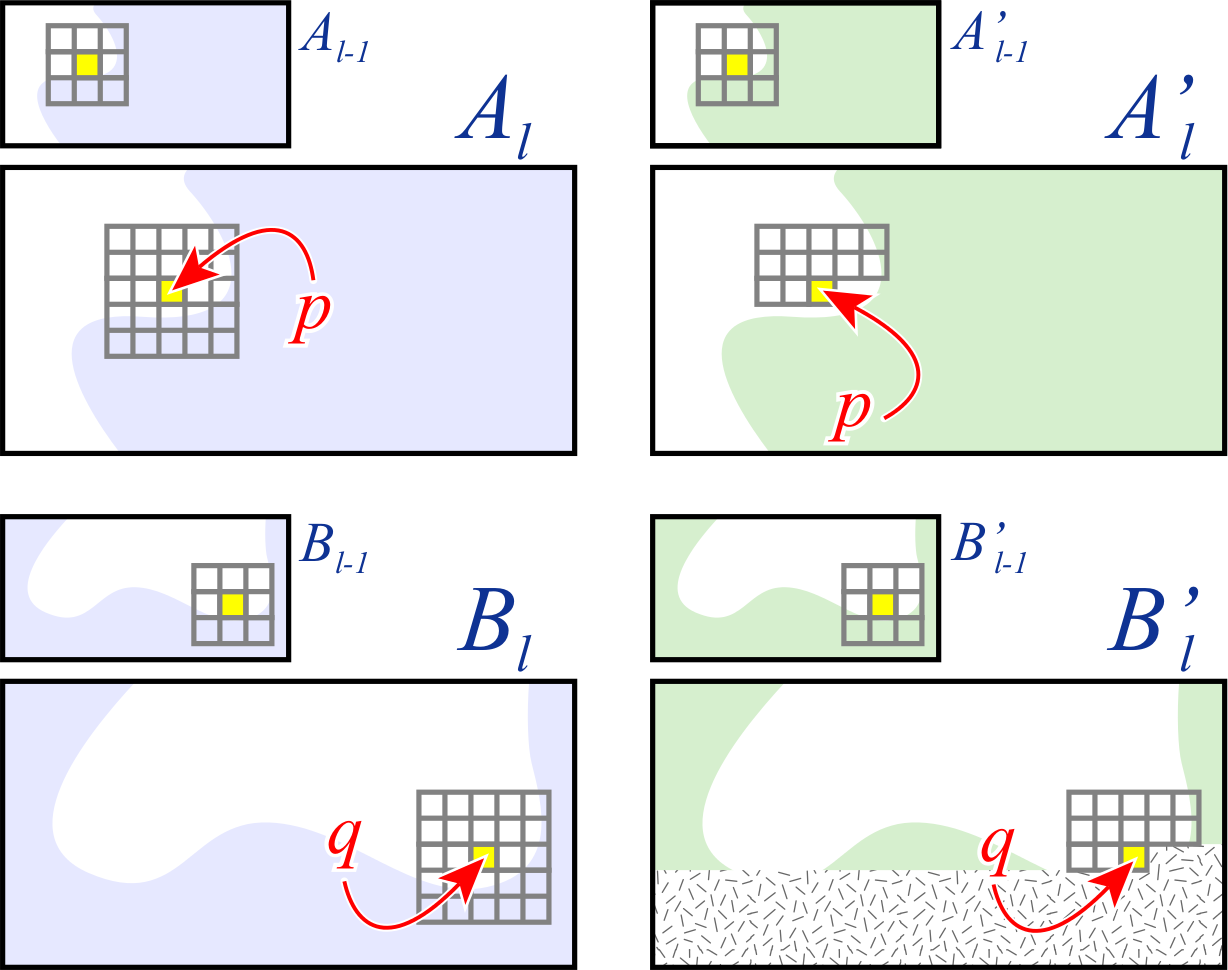
\includegraphics[width=\textwidth]{img/ia_diagram}
	\caption{ Neighbourhood matching for the Image Analogies framework, image taken from~\cite{Ashikhmin2001}.}
	\label{fig:ia_diagram}
\end{minipage}
\hfill
\begin{minipage}[b]{.4\textwidth}
\centering
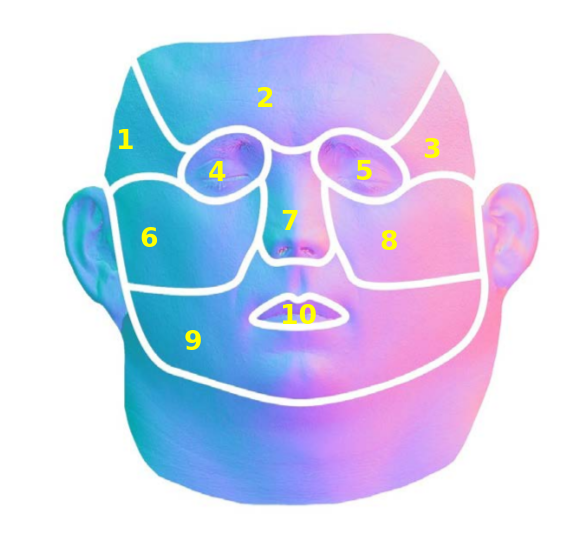
\includegraphics[width=\textwidth]{img/texture_synthesis_parts}
	\caption{ Texture segmentation in common coloured areas, image taken from~\cite{Graham2013}.}
	\label{fig:texture_synthesis_parts}	
\end{minipage}
\end{figure}

As a first approach we tried to reproduce the results for bump mapping quality increase by Graham et al~\cite{Graham2013}, results are shown in Figure~\ref{fig:bump_maps}.
The authors add an extra parameter $\alpha \in \left\lbrace 0, \ldots, 1 \right\rbrace$ to control Hertzmann's image synthesis process.
To be more precise, a match between $A$ and $\left\lbrace B,B' \right\rbrace$ will be weighted by $1 - \alpha$, and a match between $A'$ and $\left\lbrace B,B' \right\rbrace$ will be weighted by $\alpha$.
The logic behind this addition is to encourage more details of $A'$ to be included in $B'$.
The modifications required to include this addition begin by building two separated k-d trees for $A$ and $A'$, when choosing the best match both distances will be weighted as explained above and the smaller one will be chosen.
Also in the coherence match two searches will be done and weighted accordingly, and the final pixel will be chosen without further adjustments.

\begin{figure}[htbp!]
\centering
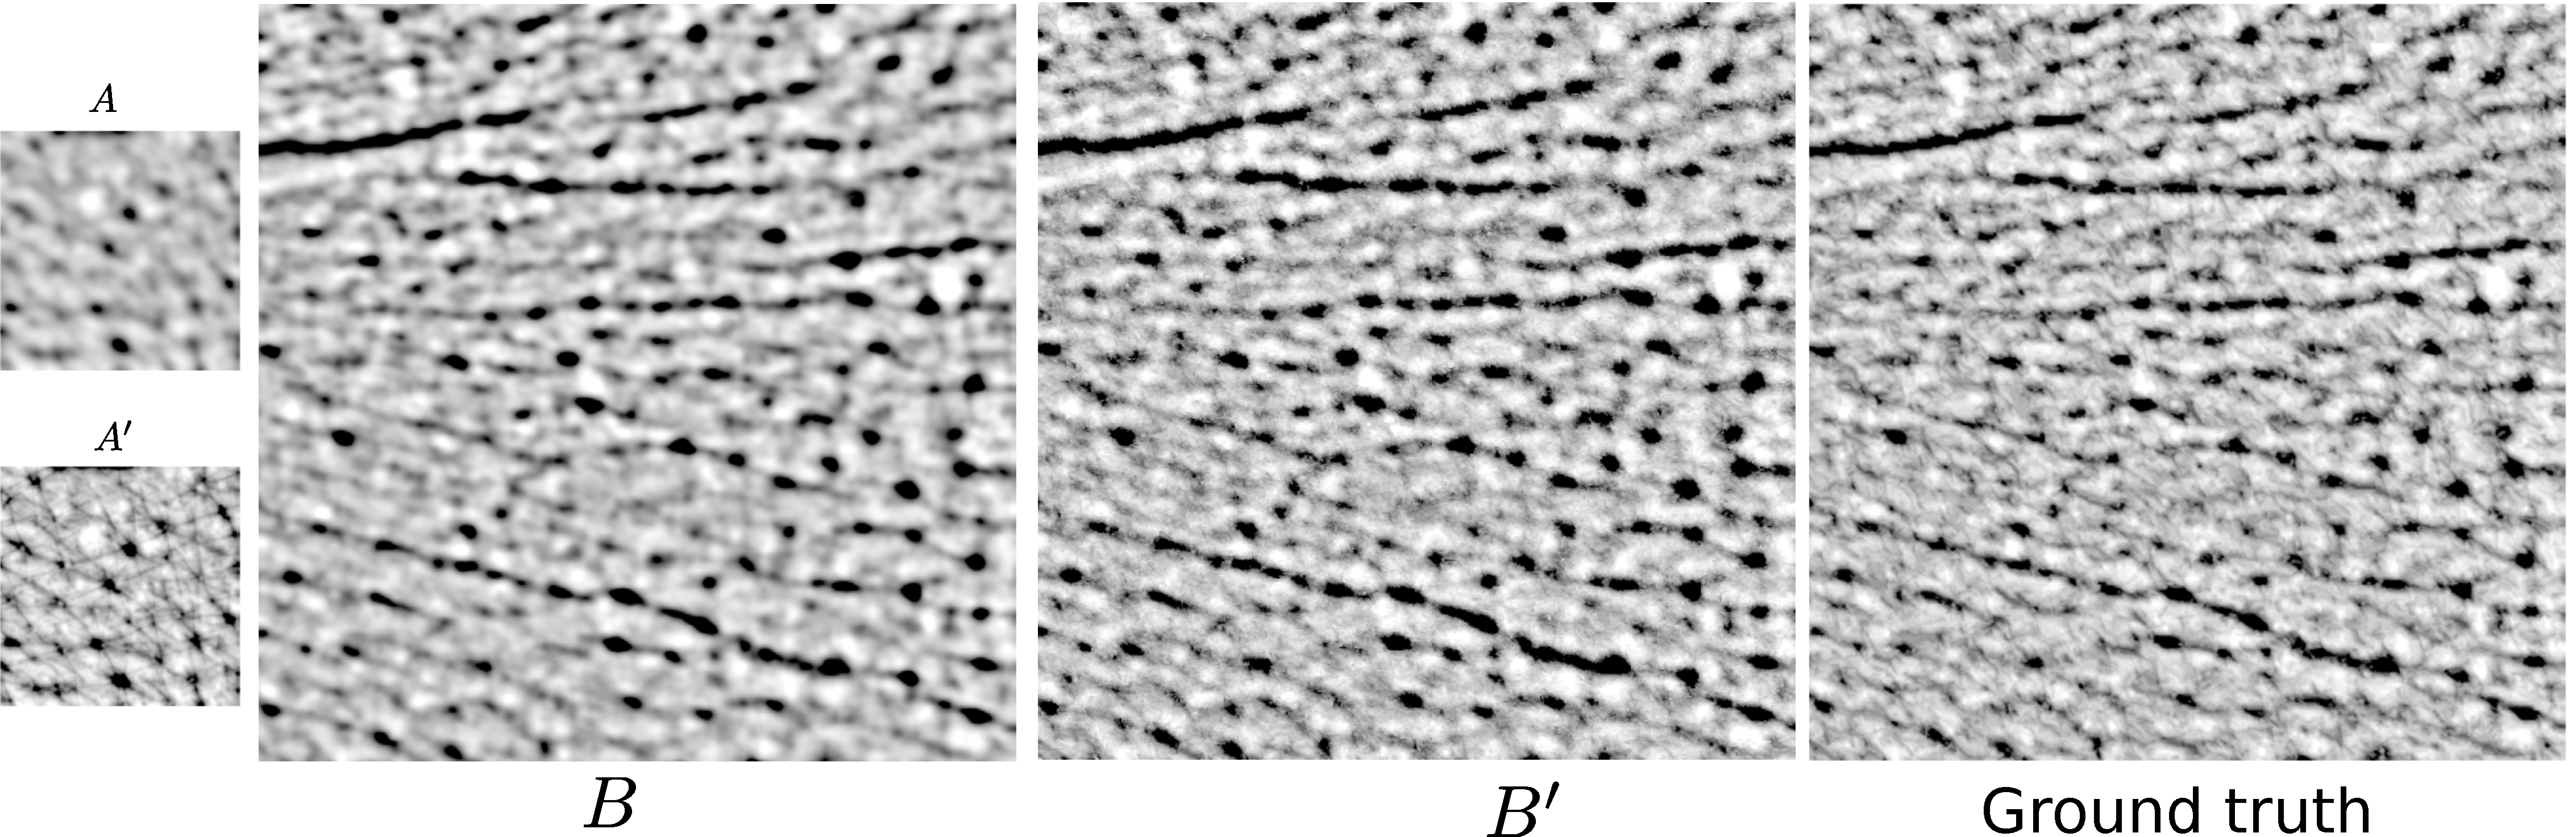
\includegraphics[width=\textwidth]{img/bump_maps}
	\caption{ Bum map deblurring, $A$, $A'$, $B$ and ground truth images images taken from~\cite{Graham2013}.}
	\label{fig:bump_maps}
\end{figure}

Another approach we tried was to use the Image Analogies filter to create increased quality textures.
The idea is to improve a low quality texture from a 3D scan using pictures of the texture taken at a closer range.
To achieve this we took a close up high quality sample $A'$, to generate $A$, the sample $A'$ was blurred using a Gaussian kernel until it look qualitative similar to the 3D scan texture $B$, with this three inputs we generated a picture $B'$ of higher quality.
Since faces have differentiated areas, this process was done separately for each of them, the generated patches are stitched together using linear interpolation.
The texture segmentation is shown in Figure~\ref{fig:texture_synthesis_parts} and results are shown in Figure~\ref{fig:texture_synthesis}.

\begin{figure}[htbp!]
\centering
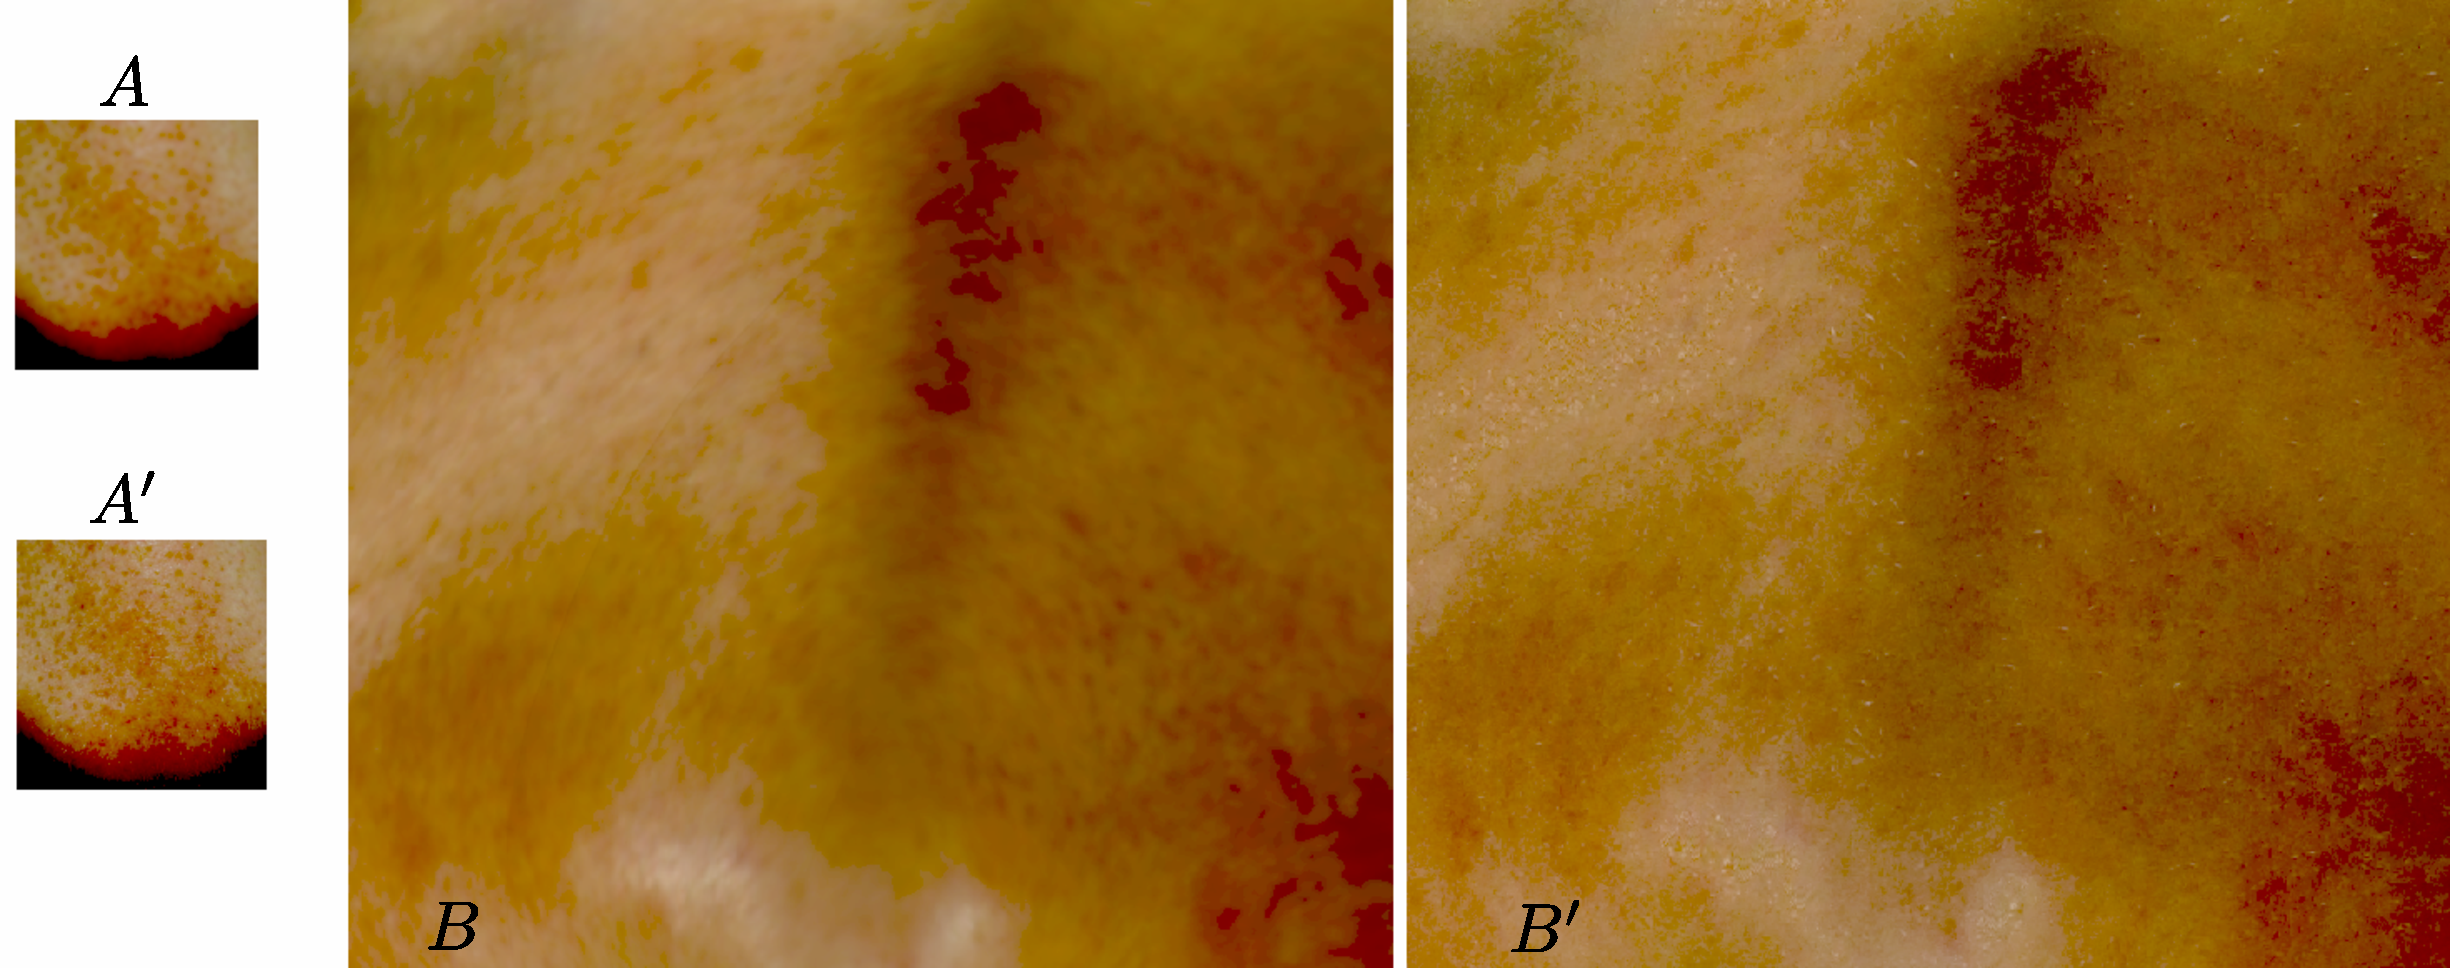
\includegraphics[width=\textwidth]{img/texture_synthesis}
	\caption{ Texture quality increase using image analogies, the texture is false-coloured to highlight the differences.}
	\label{fig:texture_synthesis}
\end{figure}

Another option for increasing the quality of the texture is to use image super-resolution, we used Jianchao et al~\cite{Jianchao2010} work for this purpose.
The idea is that by doubling the resolution of the original texture, yet avoiding blur by adding information from a dictionary of high resolution images, the final rendering quality of the face will increase.
Results for this approach are shown in Figure~\ref{fig:emily_super_resolution}.

\begin{figure}[htbp!]
\centering
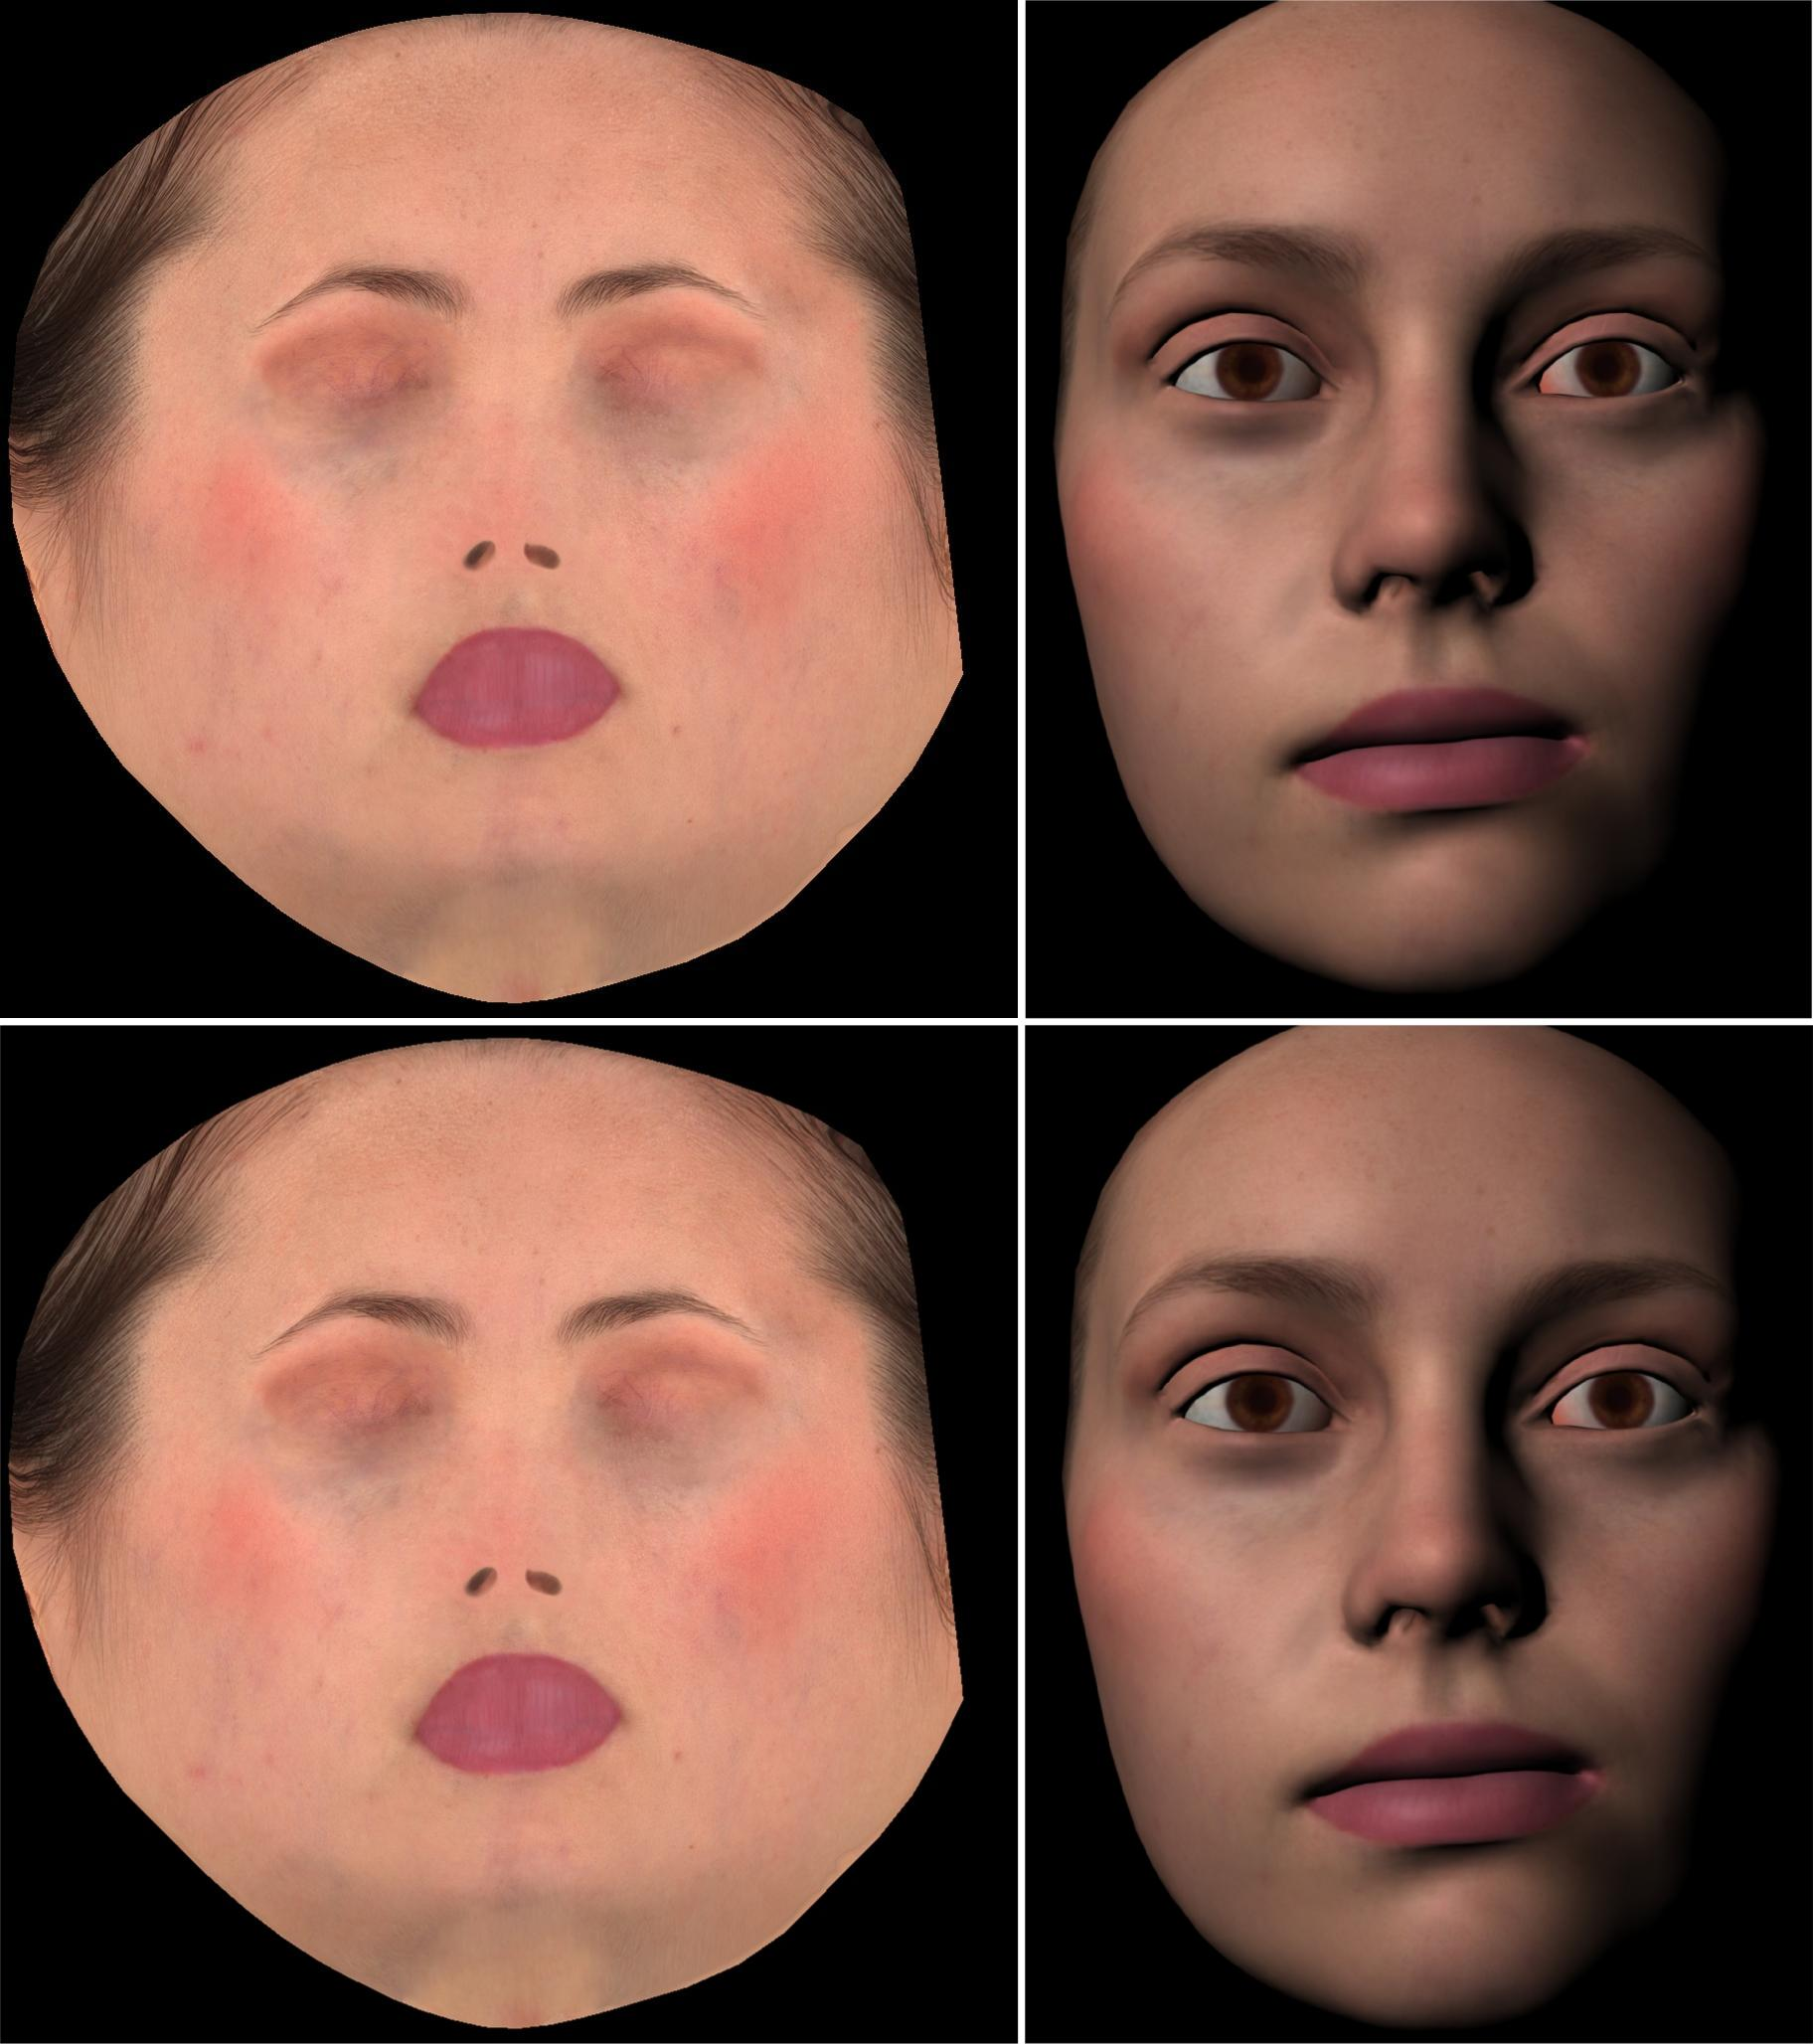
\includegraphics[width=\textwidth]{img/emily_super_resolution}
	\caption{ Super resolution example, left original texture, left-centre face rendered with original texture, right-centre super-resolution texture, right face rendered with super-resolution texture, original data from \cite{FaceWareWeb}.}
	\label{fig:emily_super_resolution}
\end{figure}

Generating normals maps using Image Analogies is another interesting area, as it could provide an alternative to the costly standard capture methods.
For this we tried to generate a normal maps from albedo images and from bump maps generated from the previous 3D scan texture, results are shown in Figure~\ref{fig:normal_synthesis}. 
To create the bump maps, the textures were transformed to gray scale and a histogram equalization was applied.
In order to improve the quality of the bump maps, we also applied the Image Analogies filter to them using a known good bump map as a filtered example, however the quality did not improve significantly.

\begin{figure}[htbp!]
\centering
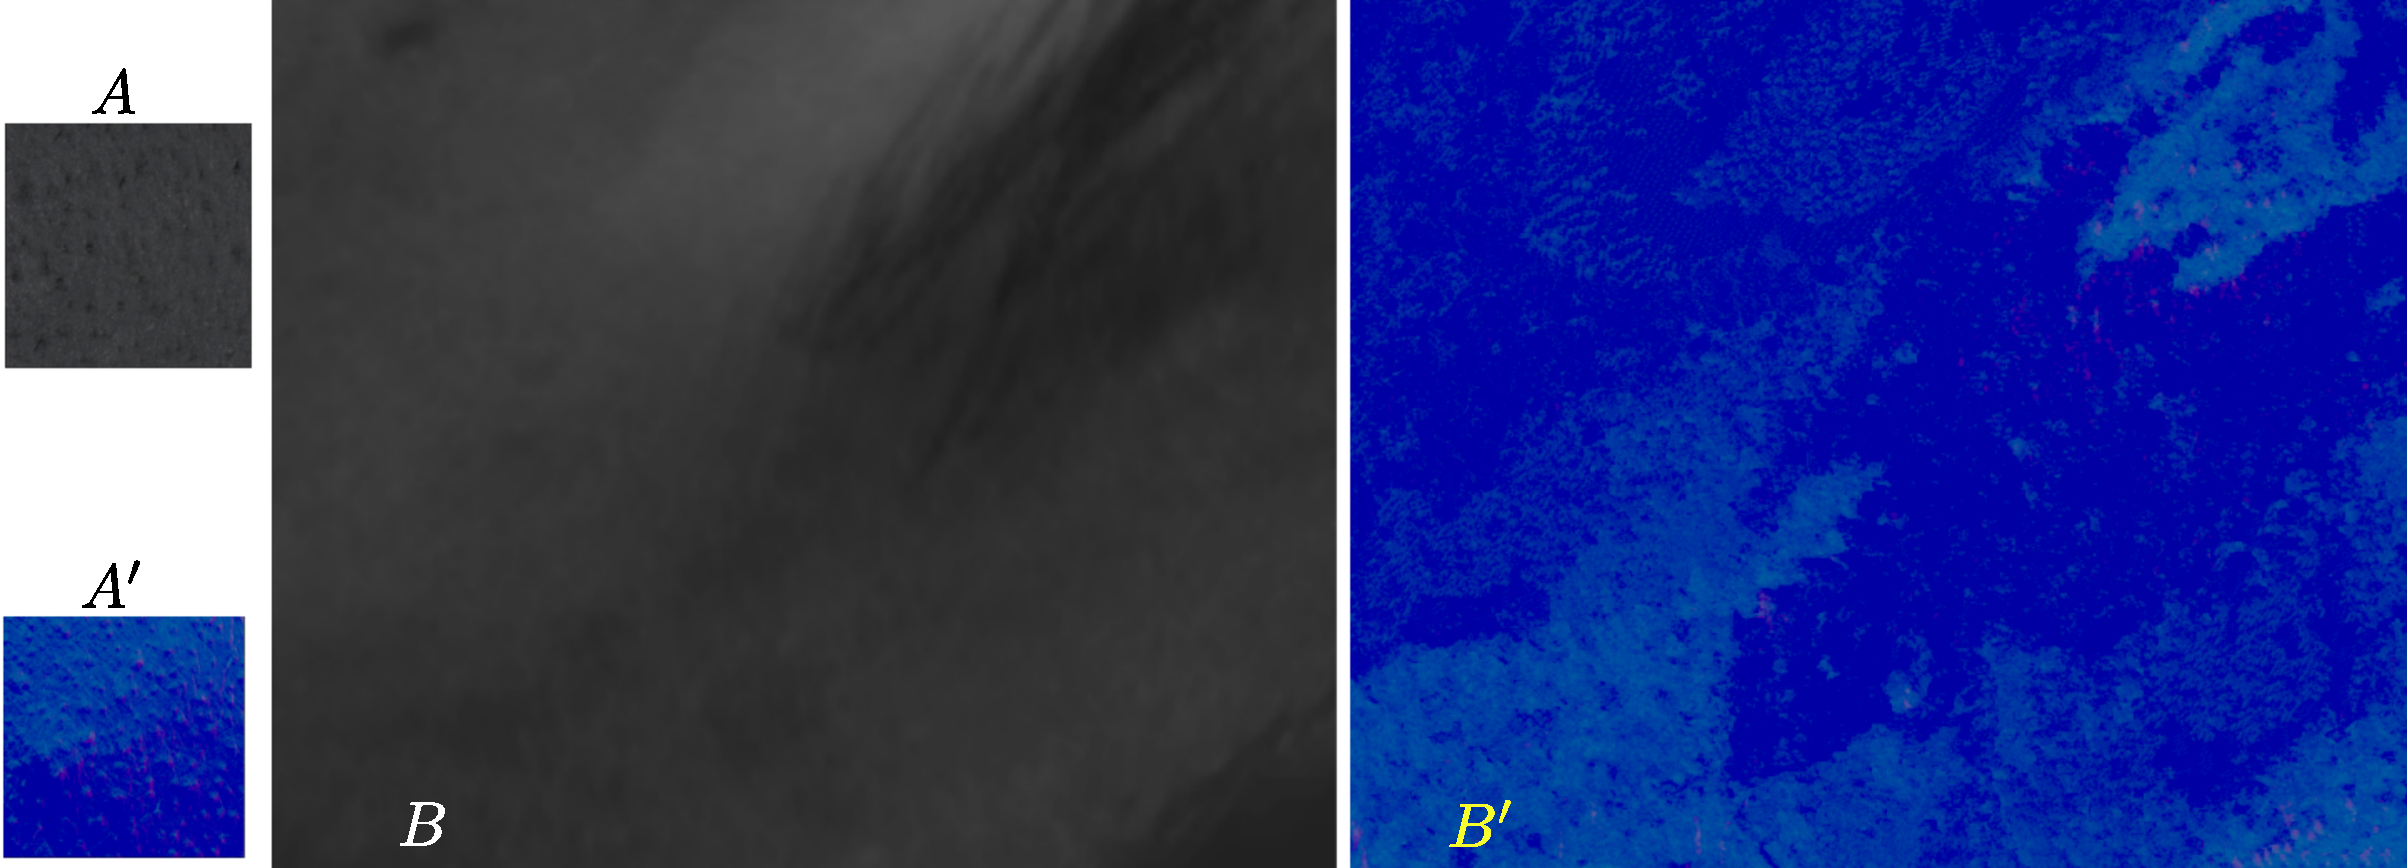
\includegraphics[width=\textwidth]{img/normal_generation}
	\caption{ Normal synthesis from albedo image.}
	\label{fig:normal_synthesis}
\end{figure}

\section{Implementation details}
\label{sec:implementation_details}

Talk about Maya plugins and any other implementation stuff worth talking about. 

%-----------------------------------------------------------------------
\section{Results}


%-----------------------------------------------------------------------
\section{Conclusions}

\bibliographystyle{eg-alpha}
\bibliography{baththesis}

\end{document}